\documentclass[12pt, a4paper]{report}

% --- FONT E TIPOGRAFIA PROFESSIONALE ---
\usepackage[utf8]{inputenc}
\usepackage[T1]{fontenc}
\usepackage{newpxtext,newpxmath}
\usepackage{microtype} 
\usepackage{xcolor}

% --- PACCHETTI STANDARD ---
\usepackage{graphicx}
\usepackage{svg}
\usepackage{fancyhdr}
\usepackage{hyperref}
\setlength{\marginparwidth}{2cm}
\usepackage{todonotes}
\usepackage{amsmath}
\usepackage{adjustbox}
\usepackage{nomencl}
\usepackage{etoolbox}
\usepackage{setspace}
% --- MARGINI ---
\usepackage[top=2cm, bottom=2.5cm, left=3cm, right=3cm]{geometry}
% --- FORMATTAZIONE CAPITOLI (titlesec) ---
\usepackage{titlesec}
\usepackage[style=numeric, sorting=none, backend=biber]{biblatex}
\addbibresource{References.bib}

\definecolor{chapgray}{gray}{0.4} % Grigio elegante per il numero del capitolo

\titleformat{\chapter}[display]
  {\normalfont\bfseries} % Formato generale
  {\raggedleft\Large\color{chapgray} \chaptertitlename\ \thechapter} % Numero del capitolo (più piccolo e grigio)
  {1ex} % Spazio tra numero e titolo
  {\titlerule\vspace{2ex}\Huge\raggedleft} % Linea separatrice e Titolo in grande
  [\vspace{-1ex}]

% --- METADATI ---
\title{Protecting the autonomic manager \\[1ex] \color{chapgray}\LARGE A comparative analysis of Quorum and CometBFT as blockchain backends for Self-Protecting Systems}
\author{Valerio Tatti}
\date{Aprile 2026}

\makeatletter
\newcommand{\myTitle}{\@title}
\newcommand{\myAuthor}{\@author}
\newcommand{\myDate}{\@date}
\makeatother
\newcommand{\myMatricola}{609824}
\newcommand{\myRelatore}{Prof. Stefano Iannucci}
\onehalfspacing 
\begin{document}

\pagenumbering{alph}
% Inserisce la nuova copertina

\begin{titlepage}
    \begin{center}
        
        % --- LOGO CENTRATO ---
        \vspace*{10mm}
        
\includegraphics[width=0.45\linewidth]{Public/Logo_RM3.png} \\[0.5cm]
        
        % --- INTESTAZIONE UNIVERSITA' CENTRATA ---
        {\LARGE \scshape Università degli Studi} \\[0.3cm]
        {\Large Dipartimento di Ingegneria Civile, Informatica\\ e delle Tecnologie Aeronautiche}

        \vspace*{24mm}

        % --- TIPO DI ELABORATO ---
        {\fontsize{18pt}{14pt}\selectfont \textbf{Tesi di Laurea}} \\
        \vspace{6mm}

        % --- TITOLO ---
        {\Huge \textbf{\myTitle}} \\
        \vspace{35mm}
        % --- GRIGLIA  ---
        \large
        \renewcommand{\arraystretch}{2} % Altezza delle righe
        \begin{tabular}{r l}
            \fontsize{14pt}{10pt}\textbf{Corso di Laurea:}  & \underline{\makebox[9cm][c]{Ingegneria Informatica}} \\
            \fontsize{14pt}{10pt}\textbf{Candidato:}        & \underline{\makebox[9cm][c]{\myAuthor}} \\
            \fontsize{14pt}{10pt}\textbf{Matricola:}        & \underline{\makebox[9cm][c]{\myMatricola}} \\
            \fontsize{14pt}{10pt}\textbf{Relatore:}         & \underline{\makebox[9cm][c]{\myRelatore}} \\
            \fontsize{14pt}{10pt}\textbf{Anno Accademico:}  & \underline{\makebox[9cm][c]{2025/2026}} \\
        \end{tabular}
        
    \end{center}
\end{titlepage}

\clearpage
\pagenumbering{roman}
\tableofcontents
\listoffigures
\listoftables

\clearpage
\pagenumbering{arabic}

% ==============================================================================
% CHAPTER 1: INTRODUCTION
% ==============================================================================

\chapter{Introduction}
\label{chap:introduction}

Modern IT infrastructures have undergone a deep transformation over the last decade. The rapid shift toward cloud-native, containerized microservices has decomposed monolithic applications into dozens of cooperating processes distributed across heterogeneous hosts, and the digital attack surface has expanded accordingly. In this landscape, cyber threats have grown in both sophistication and amount: attackers chain exploits across services, automate attacks and weaponize compromised components faster than human operators can respond. The sheer volume of sensitive data housed in these environments, and the regulatory cost of exposing it, have turned the ability to \emph{defend autonomously} from a convenience into a necessity. Within this context, the autonomic computing paradigm has become a cornerstone of modern security engineering, promising to reduce human operational burden and to compress the time between detection and response. However, while automation resolves many latency and coordination challenges, it introduces a new and subtler systemic vulnerability: if the automated security logic itself becomes the target, a single compromise can be turned into a vector for devastating privilege escalation and system-wide failure. This thesis investigates how to build the decision substrate of such an autonomous defender.

% : : : : : : : : : : : : : : : : : : : : : : : : : : 
\section{The Paradigm of Self-Protecting Systems}
\label{sec:intro_paradigm}
% : : : : : : : : : : : : : : : : : : : : : : : : : : 

Self-Protecting Systems \cite{10.1145/2555611} (SPS) are autonomic software systems designed to detect, analyze, and mitigate security threats dynamically with limited or no human intervention. They are one of the four ``self-*'' facets: alongside self-configuration, self-optimization, and self-healing: through which IBM's autonomic computing manifesto \cite{kephart2003vision} originally characterized self-managing software, and they operationalize the self-protection objective through a continuous feedback loop.

Following the classic autonomic feedback loop, an SPS typically comprises two primary macro-components: a \textit{managed system} and an \textit{autonomic manager}. The managed system represents the production environment, the services, containers, or software applications that are directly exposed to potential attacks. Conversely, the autonomic manager serves as the central controller responsible for executing the security loop, and its internal logic is structured around the MAPE-K cycle \cite{kephart2003vision, 7194653}: it \emph{monitors} the managed system through sensors, \emph{analyzes} the collected observations, \emph{plans} a response consistent with high-level policies, and \emph{executes} it through effectors, all grounded on a shared \emph{knowledge} base.

To achieve continuous protection, the autonomic manager organizes its operations into a pipeline governed by two main functional sub-components:
\begin{itemize}
    \item \textbf{Intrusion Detection Systems (IDS):} Passive or active security sensors distributed across the managed system to monitor traffic, logs, or system calls and detect anomalous behavior or known attack signatures.
    \item \textbf{Intrusion Response Systems (IRS):} Decision-making engines responsible for selecting and executing the appropriate response actions (countermeasures) to neutralize or mitigate the detected threats.
\end{itemize}

In a self-protecting loop, the quality of protection is therefore bounded by two coupled properties: the correctness and diversity of the observations that the IDS plane produces, and the timeliness and integrity with which the IRS plane turns those observations into enforced countermeasures. The work of this thesis concentrates on the latter: not on how attacks are detected, but on whether the decision substrate that sits between detection and actuation can be trusted to remain correct, responsive, and available even when the infrastructure around it is under active attack.

% : : : : : : : : : : : : : : : : : : : : : : : : : : 
\section{The Vulnerability of the Autonomic Manager}
\label{sec:intro_vulnerability}
% : : : : : : : : : : : : : : : : : : : : : : : : : : 

Although highly effective in mitigating threats directed at the managed system, this canonical design suffers from a critical structural vulnerability: the centralization of the autonomic manager. An adversary who penetrates the infrastructure can target the autonomic manager itself. By compromising this central controller, the attacker can silence intrusion alerts, disable response mechanisms, or even manipulate the manager into executing malicious countermeasures (e.g., disconnecting legitimate network segments or isolating critical database services).

This is the ``Who watches the watchers?'' dilemma of autonomic computing \cite{chess2003security, pekaric2023systematic}: the very component that is supposed to enforce security becomes a high-value target, and protecting it through conventional defense-in-depth only hardens a single point of failure rather than removing it. If the security logic is centralized and compromised, the integrity of the entire infrastructure is undermined, rendering the self-protecting features not only ineffective but actively weaponized against the system. The state of the art has explored several responses to this dilemma, each with its own limitations. Traditional hardening of a centralized manager \cite{pekaric2023systematic} reduces the attack surface but does not eliminate the single point of failure. Trusted Execution Environments (TEEs), and in particular Intel SGX, have established themselves as the current benchmark by executing the manager's critical logic inside a hardware enclave; yet they remain exposed to microarchitectural side-channel attacks such as Spectre, Meltdown, and ZombieLoad, they introduce vendor lock-in, and, crucially, they do not solve the availability problem, since an attacker can simply crash or disconnect the single host running the enclave. A structural solution is therefore needed; one that removes the centralization assumption altogether rather than reinforcing it.

% : : : : : : : : : : : : : : : : : : : : : : : : : : 
\section{Blockchain as a Mechanism of Trust}
\label{sec:intro_blockchain}
% : : : : : : : : : : : : : : : : : : : : : : : : : : 

To eliminate the single point of failure represented by a centralized manager, our research \cite{11126595} has proposed distributing the autonomic manager across a permissioned blockchain network. In this decentralized architecture, blockchain technology acts as a tamper-proof ledger and a distributed state machine (DSM) that logs security events and executes response logic securely. Replicating the manager's state across multiple independent nodes, and encoding the response logic as a deterministic transition function over a globally agreed state, converts the manager from an isolated, hardening-dependent process into a resilient, physically separated network whose correctness rests on a formal fault model rather than on the impregnability of a single host.

This distributed approach establishes fundamental security guarantees that collectively safeguard the autonomic loop. To prevent a single compromised IDS sensor from injecting false alerts and triggering unauthorized countermeasures, the state machine enforces a consensual voting mechanism. Under this scheme, updates to the shared security state are only committed once they receive corroborating reports from multiple independent, heterogeneous IDSs, ensuring that isolated sensor compromises do not lead to malicious actuations.

Also, by deploying the autonomic manager across a network of validator nodes running a Byzantine Fault-Tolerant (BFT) consensus protocol, the security loop gains strong structural resilience. At blockchain level, this mechanism tolerates the active compromise of up to $1/3$ of validators while preserving ledger safety and finality under partial network compromise. This guarantee is distinct from IDS-side voting, which is the mechanism used to validate the semantic correctness of observations before they affect the consolidated monitored state. The two layers compose into a two-threshold fault model: an attacker must subvert either a majority of the heterogeneous IDSs observing a variable or a supermajority of the consensus validators, a requirement that makes the compromise of the autonomic manager highly improbable.

Generally, the system is designed to reduce the attack surface as much as possible by treating actuators as black boxes (blind). The actuators receive signed mitigation commands directly from the blockchain state, rather than querying the state of potentially compromised application containers directly. This enforces a strict unidirectional data flow: IDSs push observations to the consensus plane, the blockchain validates and commits the state transition, and the resulting response is pushed to the actuators: so that an actuator only ever executes commands that have passed through BFT consensus.

A final, often overlooked, property is \emph{deterministic finality}. A software control loop cannot act on decisions that might subsequently be rolled back, so the underlying consensus must commit blocks that are final and immutable rather than probabilistically finalized. This rules out the public, permissionless blockchain model and its Proof-of-Work/Proof-of-Stake machinery, with their tokenomics, high latency, and resource consumption, and it motivates the choice of a permissioned environment where participants are pre-vetted, identities are static, and consensus can be simplified to a BFT protocol with immediate finality.

% : : : : : : : : : : : : : : : : : : : : : : : : : : 
\section{The Technology Choice Is Not Neutral}
\label{sec:intro_tech_choice}
% : : : : : : : : : : : : : : : : : : : : : : : : : : 

While the theoretical integration of blockchain into the SPS architecture provides outstanding security guarantees, the practical choice of the underlying blockchain technology is not neutral. A blockchain-based autonomic manager has unique requirements: it must handle sparse, highly event-driven alert traffic with exceptionally low latency and high determinism, and it must absorb bursty, redundant alert storms without collapsing into unbounded latency or silently dropping observations. Conversely, many features native to public blockchains: virtual-machine-level gas metering, token economics, transaction fees, dynamic peer discovery, and an archival storage model: add unnecessary complexity, expand the trusted computing base (TCB), and increase the attack surface without contributing to the control loop.

The natural baseline choice for permissioned enterprise setups is GoQuorum, a fork of Ethereum that retains the Ethereum Virtual Machine (EVM) and provides BFT consensus through IBFT/QBFT. However, this thesis argues that general-purpose smart-contract platforms incur severe, non-intrinsic performance overheads due to interpreted virtual machine bytecode execution, rigid transaction fee mechanisms, and fixed-interval block production: every alert pays RLP serialization, EVM bytecode interpretation, and instruction-granularity gas metering that execute unconditionally even though fees are zero, and the fixed block period caps how quickly the mempool can drain. As an alternative, this work explores CometBFT (the successor of Tendermint), a lower-level BFT consensus engine that keeps consensus separate from the application and supports highly optimized, application-specific distributed state machines through the Application BlockChain Interface (ABCI). In CometBFT the SPS state machine can be implemented as a native function call, empty blocks can be disabled so that the first transaction is proposed immediately, and the runtime cost of a state transition becomes proportional to its intrinsic logic rather than to virtual-machine scaffolding.

The comparison is framed through a deliberately requirement-driven lens: a feature that is not needed by the SPS manager is best \emph{absent}, because any additional subsystem increases configuration complexity, wastes computational power, and creates new failure modes or attack vectors that must themselves be secured. Under this lens, the absence of non-required functionality in CometBFT is itself a form of alignment with the SPS use case.

% : : : : : : : : : : : : : : : : : : : : : : : : : : 
\section{Objectives and Contributions of the Thesis}
\label{sec:intro_objectives}
% : : : : : : : : : : : : : : : : : : : : : : : : : : 

The primary objective of this thesis is to present a comprehensive qualitative and empirical comparison between a conventional general-purpose platform (GoQuorum) and a requirement-driven, application-specific alternative (CometBFT) to determine which architecture best supports the performance and cyber-resilience demands of modern Self-Protecting Systems. The comparison is requirement-driven rather than feature-driven: it does not reward a platform for offering additional services unless those services directly improve the SPS manager's correctness, latency, or operational resilience.

Specifically, the core contributions of this thesis are as follows:
\begin{enumerate}
    \item \textbf{Requirement Formulation:} We define and classify a comprehensive set of functional and non-functional requirements (required, desirable, and not needed) for blockchain technology in the specific context of an autonomic SPS loop, derived from the architecture and aligned with the fixed trust boundary of a permissioned deployment.
    \item \textbf{Architectural Analysis:} We conduct a thorough qualitative comparison of GoQuorum and CometBFT, highlighting the architectural mismatch of general-purpose virtual machines versus application-specific state machines, and reading each platform's design choices onto the SPS requirement set.
    \item \textbf{Prototype Implementation:} We design and implement a realistic, fully containerized SPS prototype emulated via Kathará on top of Docker. The prototype integrates three heterogeneous IDS engines (Snort, Suricata, and Zeek) protecting a vulnerable web application (OWASP Juice Shop), and runs interchangeably on both blockchain backends so that any measured difference is attributable to the consensus substrate.
    \item \textbf{Deduplication Middleware:} We propose and develop a custom deduplication middleware layer for the member nodes. This layer filters repetitive alerts before they reach the mempool, collapsing temporally adjacent observations that request the same state transition into a single on-chain transaction and keeping the transaction count upper-bounded per block.
    \item \textbf{Empirical Evaluation:} We perform extensive automated benchmarks under controlled attack conditions, comparing GoQuorum and CometBFT across key performance indicators: end-to-end response latency, transaction throughput under heavy load, and the compression ratio achieved by the deduplication middleware: and relate the measured behaviour back to the qualitative predictions of the requirement analysis.
\end{enumerate}

% : : : : : : : : : : : : : : : : : : : : : : : : : : 
\section{Structure of the Thesis}
\label{sec:intro_structure}
% : : : : : : : : : : : : : : : : : : : : : : : : : : 

To thoroughly explore the theoretical background, architectural design, and empirical evaluation of the proposed systems, the remainder of this thesis is structured as follows:

\begin{description}
    \item[Chapter 2 -- Technologies Setting and Related Work:] Introduces the foundational concepts of autonomic computing and the MAPE-K cycle, the structure of permissioned blockchain environments, the family of distributed consensus algorithms from Crash Fault Tolerance to Byzantine Fault Tolerance, and reviews the state of the art in autonomic manager security, from traditional hardening to Trusted Execution Environments and distributed ledger technologies.
    \item[Chapter 3 -- A Cyber-Resilient Architectural Model:] Details the technology-agnostic architecture of the Self-Protecting System, formalizing the system decomposition into detection, consensus-and-decision, and control planes, the replicated state machine that governs the autonomic loop, the end-to-end protection workflow, and the safety, liveness, and threat-model properties that the architecture guarantees.
    \item[Chapter 4 -- Requirement Alignment: Quorum vs. CometBFT:] Formally identifies the blockchain properties strictly required, desirable, and not needed for SPS applications, and theoretically compares Quorum's general-purpose execution environment with CometBFT's application-specific design through a requirement-alignment table.
    \item[Chapter 5 -- Implementation Details:] Describes the prototype implementation, the containerized network topology emulated via Kathará, the realization of the replicated decision state machine as both a Solidity contract and a Rust ABCI application, the end-to-end alert response loop, and the custom deduplication middleware developed for the evaluation.
    \item[Chapter 6 -- Experiments and Results:] Analyzes the performance of the two blockchain backends under three research questions: end-to-end latency under low traffic, sustained throughput under increasing load, and the effectiveness of the deduplication middleware: presenting metrics on response time, transaction throughput, and the compression of redundant attack traffic.
    \item[Chapter 7 -- Conclusions and Future Work:] Summarizes the findings of the comparative analysis, acknowledges the limitations of the study in terms of experimental setting, threat-model scope, and engineering maturity, and outlines directions for future research including physical cluster deployments, richer attack scenarios, sharding, and formal verification of the state transition function.
\end{description}

% ==============================================================================
% CHAPTER 2: TECHNOLOGIES SETTING
% ==============================================================================

\chapter{Technologies Setting and Related Works}
\label{chap:technologies}
% Introduce the background concepts necessary to understand the thesis.
Before diving into the specific idea and implementation behind the system described in this research, it is necessary to introduce the basic theoretical concepts that inspired this architecture. These concepts will later provide us with the tools to comprehend by which metrics a blockchain-based autonomic agent should be measured, which paradigm first described autonomic systems, which security issues we can expect, how the current state-of-the-art (SOTA) solutions address them, and how our architecture compares to them.

\section{Autonomic Computing and the MAPE Cycle}
\label{sec:tech_autonomic}
The paradigm of Autonomic Computing formally emerged in October 2001, when IBM released a manifesto identifying an upcoming software complexity crisis as the primary obstacle to further progress in the IT industry~\cite{kephart2003vision}. As computing environments began to weigh in at millions of lines of code, the expertise required for installation, configuration, and maintenance approached a limit on human capability to train new professionals. This challenge was exacerbated by the necessity of integrating several heterogeneous environments into corporate-wide systems and extending them globally across the Internet. IBM observed that relying solely on innovations in programming methods would not suffice to manage such massive and complex systems, which often require timely responses to rapid streams of changing demands.

To address this problem, IBM proposed the vision of autonomic computing: systems capable of managing themselves based on high-level objectives from human administrators~\cite{kephart2003vision}. The term "autonomic" was chosen for its biological connotation, tracing an analogy to the human autonomic nervous system. Just as the biological system governs vital, low-level functions such as heart rate and body temperature without conscious effort, autonomic computing aims to free human administrators from the burden of managing low-level system operations through automation.

\subsection{The Four Aspects of Self-Management}
The essence of autonomic computing is self-management, intended to provide software that can adjust its behaviour in accordance with human objectives without their intervention~\cite{kephart2003vision}. IBM characterizes self-management through four fundamental aspects, often referred to as the "self-*" properties. Those principles have since materialized into concrete industry standards and architectural paradigms that govern contemporary network infrastructures:

\begin{itemize}
    \item \textbf{Self-configuration}: Systems must automatically configure components and integrate themselves into complex environments following high-level policies. New components should be able to incorporate seamlessly, treating other components as black boxes. This modular perspective prefigured modern containerization paradigms, where container runtimes such as Docker have become the industry standard for application deployment.
    \item \textbf{Self-optimization}: Autonomic systems continually seek opportunities to improve their own performance and efficiency. In environments like complex middleware or databases that possess hundreds of manually set parameters, the system must monitor, experiment with, and tune these parameters dynamically. A notable industrial implementation of this concept is cloud-based auto-scaling (e.g., Amazon Web Services Auto Scaling), which dynamically adjusts resource provisioning to match fluctuating performance demands.
    \item \textbf{Self-healing}: The system is designed to automatically detect, diagnose, and repair localized software and hardware problems. Using knowledge of the system configuration and logs, the autonomic manager can identify root causes of failures, match them against known patches, and retest the system without manual debugging. In contemporary orchestration systems, self-healing is commonly implemented via automated health checks and liveness probes (e.g., in Kubernetes), which automatically restart or replace failing service instances.
    \item \textbf{Self-protection}: Autonomic systems defend the infrastructure as a whole against malicious attacks~\cite{yuan2014systematic}. They use sensor reports to anticipate problems and take proactive steps to avoid or mitigate systemwide failures. An example of such proactive defense is represented by modern Web Application Firewalls (WAFs), such as Cloudflare’s edge security systems, which autonomously detect, analyze, and block malicious traffic patterns.
\end{itemize}


\subsection{The Structure of Autonomic Elements}
Architecturally, autonomic systems are composed of elements that manage their own internal behavior and relationships with others in accordance with established policies~\cite{kephart2003vision}. An autonomic element typically consists of one or more managed elements coupled with a single autonomic manager.

\begin{itemize}
    \item \textbf{Managed Element}: This component can be found in non-autonomic systems and can be a hardware resource (such as storage or a CPU) or a software resource (such as a database or a web service).
    \item \textbf{Autonomic Manager}: The manager distinguishes the autonomic element by monitoring the managed element and its environment, and executing actions based on the analysis of their information.
\end{itemize}

The internal logic of the autonomic manager is structured around a fundamental control loop known as the \textbf{MAPE-K} cycle~\cite{kephart2003vision, 7194653}:
\begin{enumerate}
    \item \textbf{Monitor}: Collects, aggregates, and filters information from the managed element and its environment.
    \item \textbf{Analyze}: Matches a diagnosis on the system's high-level status based on monitored information and triggers a response.
    \item \textbf{Plan}: Creates or selects a sequence of actions that matches the organization's objectives.
    \item \textbf{Execute}: Applies the derived plan / action to the managed element through effectors.
    \item \textbf{Knowledge}: A central repository for policies, historical data, and system configurations that supports the other four phases defining the organization's objectives.
\end{enumerate}

\subsection{Security Challenges}
Autonomic elements, unlike typical Web services, do not honor requests unconditionally; they provide services only if doing so is consistent with their internal goals~\cite{kephart2003vision}.

This high degree of autonomy introduces critical system-level issues that cannot be ignored when evaluating attack surfaces. Because these systems rely on high-level goals, they are vulnerable to new forms of attack where an adversary might manipulate policies to gain systemic leverage~\cite{chess2003security}. This highlights the necessity for a secure-by-design management infrastructure that can address the "Who watches the watchers?" dilemma of autonomic elements~\cite{chess2003security, pekaric2023systematic}.

\section{Blockchain in Permissioned Environments}
\label{sec:tech_permissioned_blockchain}

The integration of blockchain technology to register system state represents an innovative approach to ensuring cyber-resilience~\cite{11126595}. However, in this specific application context, the choice of the underlying blockchain platform is not neutral, and it is necessary to define which blockchain properties are beneficial for a Self-Protecting System. A fundamental distinction must be made between public (permissionless) blockchains and private (permissioned) blockchains~\cite{wang2022bft}.

\subsection{Smart Contracts and Response Logic}
Before analyzing network access models, it is essential to define the mechanism through which the blockchain enforces security policies: the \textit{smart contract}. A smart contract is a self-executing distributed software deployed on a blockchain that automatically enforces predefined rules and agreements between nodes without the need for intermediaries~\cite{buterin2013ethereum}.

Once deployed, smart contracts run deterministically across all nodes in the network, ensuring the transparency, trustlessness, and immutability of the encoded logic~\cite{buterin2013ethereum}. In the context of a Self-Protecting System (SPS), the integrity of the smart contract's state and its execution is guaranteed by the inherent properties of the blockchain itself~\cite{11126595}. This enables the autonomic manager to maintain a consistent, system-wide view and coordinate responses even under partial compromise~\cite{11126595}.

\subsection{Characteristics of Permissioned Environments}
Public blockchains are designed as open networks where anyone can participate. In contrast, a permissioned environment requires nodes to authenticate each other, often within a fixed trust boundary~\cite{wang2022bft}. This architectural difference fundamentally alters the threat model and the system's performance requirements.

In a permissioned network, many attacks traditionally critical for permissionless blockchains, such as Sybil and Eclipse attacks, are naturally mitigated because participant identities are controlled and membership is typically static~\cite{11126595}.

Since permissionless environments adopt a fundamentally "trustless" model, they must employ strict, and often resource-expensive, consensus algorithms. In a permissioned blockchain, consensus can be simplified because all participating nodes are pre-vetted, identified, and operate within a predefined deployment. Consequently, the economic dynamics, gas fees, token incentives, and game-theory mechanisms typical of public cryptocurrencies designed to coordinate anonymous actors become functionally obsolete~\cite{albero2026blockchain}. Furthermore, general-purpose virtual machines (VMs) such as the Ethereum Virtual Machine (EVM) often introduce unnecessary complexity, processing overhead, and a broader attack surface when the system only requires a constrained, deterministic runtime for state transitions~\cite{albero2026blockchain}.

Instead, the focus in such environments shifts towards a specific set of essential properties. As highlighted in recent literature evaluating blockchain implementations for Self-Protecting Systems~\cite{albero2026blockchain}, the required features are:
\begin{itemize}
    \item \textbf{Byzantine Fault-Tolerant (BFT) consensus with strong finality}: To tolerate a bounded number of compromised nodes and commit updates deterministically.
    \item \textbf{Static permissioned membership}: To match the fixed trust boundary of the deployment.
    \item \textbf{Cryptographic transaction signing}: To ensure the authenticity and accountability of alerts submitted by IDSs.
    \item \textbf{Event-driven block production}: To optimize resource usage by generating blocks only when pending transactions (e.g., security alerts) are present, rather than continuously producing empty blocks during idle periods.
\end{itemize}

Additionally, desirable properties include in-memory replicated state handling (as the shared state in an SPS is typically small), low and predictable latency to guarantee timely countermeasures, and push-based notifications to immediately trigger actuators upon state updates~\cite{albero2026blockchain}.

\subsection{Alignment with SPS Requirements}
For an SPS, the blockchain's sole functions are:
\begin{itemize}
    \item To gather a shared state from Intrusion Detection Systems (IDS)~\cite{11126595}.
    \item To ensure the reliable functioning of the response logic even in the presence of security faults in the managed system or in the autonomic manager~\cite{11126595}.
    \item To communicate the response logic's decisions to the actuators securely~\cite{11126595}.
\end{itemize}

Under these assumptions, permissioned environments offer indispensable advantages, such as static membership that matches the trust boundaries of a real-world deployment~\cite{albero2026blockchain}. Furthermore, cryptographic transaction signing ensures the authenticity and accountability of sensor submissions~\cite{11126595, albero2026blockchain}. Finally, while blockchain provides an immutable audit trail for forensics, permissioned settings may allow for configurable data-retention policies, which is particularly relevant for resource-constrained or embedded systems~\cite{albero2026blockchain}.

Ultimately, the relevant blockchain properties in this domain are not openness or tokenization, but minimality, determinism, and resilience~\cite{albero2026blockchain}.
\section{Distributed Consensus Algorithms}
\label{sec:tech_consensus}

\section{State of the Art in Protecting the Manager}
\label{sec:tech_state_of_art}
% Review alternative approaches (e.g., TEEs, SGX) and their limitations.
% ==============================================================================
% CHAPTER 3: SELF-PROTECTING SYSTEMS ARCHITECTURE
% ==============================================================================

\chapter{A Cyber-Resilient Architectural Model}
\label{chap:sps_architecture}

% Present the technology-agnostic architecture based on the referenced papers.

\section{Architecture Overview}
\label{sec:sps_overview}
% Describe the managed system, manager system, IDSs, and actuators.

\section{State Representation and Response Logic}
\label{sec:sps_state_logic}
% Explain how the state-action map works.

\section{Distributed Voting Mechanism}
\label{sec:sps_voting}
% Detail how multiple sensors reach a consensus to avoid single-sensor compromise.

\section{Threat Model}
\label{sec:sps_threat_model}
% Formally define attacker capabilities, container isolation, and blind actuators.
% ==============================================================================
% CHAPTER 4: REQUIREMENTS ASSESSING
% ==============================================================================

\chapter{Requirement Alignment: Quorum vs. CometBFT}
\label{chap:requirements}

% This is the theoretical core of the comparison.

\section{Specific Requirements for SPS Applications}
\label{sec:req_sps_needs}
% Analyze what is actually needed (e.g., BFT, event-driven blocks) and what is not (Gas, PoW).

\section{Analysis of GoQuorum}
\label{sec:req_quorum}
% Discuss the legacy approach, EVM overhead, and fixed-interval block production.

\section{Analysis of CometBFT}
\label{sec:req_cometbft}
% Discuss the Distributed State Machine approach, ABCI interface, and native execution.

\section{Architectural Comparison}
\label{sec:req_comparison}
% Synthesize the mismatch/match of both technologies against the SPS requirements.

% ==============================================================================
% CHAPTER 5: IMPLEMENTATION DETAILS
% ==============================================================================

\chapter{Implementation Details}
\label{chap:implementation}

The previous chapters established, in a technology-agnostic way, the architecture of a blockchain-based Self-Protecting System (SPS) and the requirement-driven rationale for comparing Quorum and CometBFT as its decision substrate. This chapter answers the question that naturally follows: \emph{how is that abstract model actually implemented, and how can we create a fair comparison between them with real attack traffic?}

The prototype we developed ~\cite{repo} is a fully containerized, docker based system in which a real vulnerable web application is protected by three heterogeneous IDSs coordinated by a permissioned  BFT ledger. The same project can run in two setting, one on GoQuorum (QBFT) and one on CometBFT, so that every non-trivial component is exercised against both backends under identical conditions. The guiding engineering goals are: 
- structural fidelity to the architecture of Chapter~\ref{chap:sps_architecture} (every container maps to a model role, trust boundaries enforced by network isolation); 
- backend interchangeability (identical detection and control planes, so that any measured difference is attributable to the consensus substrate); 
- deterministic decision logic (identical outputs on every honest replica); 

The recurring theme of the chapter is that the two implementations are \emph{semantically equivalent} at the level of the formal state machine of Section~\ref{sec:formal_state_model}, but \emph{structurally different} in how that state machine is hosted, encoded, and scheduled. This divergence is precisely what the empirical evaluation of Chapter~\ref{chap:experiments} will measure.

\section{Emulated Network Topology and Trust Boundaries}
\label{sec:impl_topology}

The whole system is emulated with Kathará~\cite{kathara}, a lightweight Docker-based network emulator that preserves the full container isolation primitive on which the threat model of Section~\ref{subsec:security_objectives} relies: the container boundary is the primary security perimeter, and there is no shared namespace between the manager and the managed system. The topology is partitioned into six isolated segments, each enforcing a distinct trust boundary (Table~\ref{tab:topology}, conceptually depicted in Figure~\ref{fig:setting}).

\begin{table}[t]
\centering
\caption{Network segments of the SPS lab}
\label{tab:topology}
\renewcommand{\arraystretch}{1.15}
\begin{tabularx}{\linewidth}{
  >{\raggedright\arraybackslash}p{3.1cm}
  >{\raggedright\arraybackslash}p{2.5cm}
  >{\raggedright\arraybackslash}X
}
\toprule
\textbf{Segment} & \textbf{CIDR} & \textbf{Role / Trust boundary} \\
\midrule
Untrusted zone & 192.168.1.0/24 & Internet-facing; hosts the attacker only. \\
DMZ            & 10.0.0.0/24     & Managed system (Juice Shop); untrusted by assumption. \\
Management nets & 172.16.1--3.0/24 & One per IDS$\leftrightarrow$member/light pair; carries alerts only. \\
Actuator net   & 172.16.4.0/24   & Carries committed actions to the blind actuator. \\
Feedback net   & 10.0.100.0/24   & Carries NEGATIVE alerts from the actuator back to the IDSs. \\
Blockchain net & 10.99.0.0/24    & Validators, member/light nodes and full node; isolated from the DMZ. \\
\bottomrule
\end{tabularx}
\end{table}

A router container performs NAT between the untrusted zone and the DMZ and, crucially, mirrors all inbound DMZ traffic to the sniffing interfaces of the three IDSs. This mirroring decouples detection from the data path of the application: the IDSs observe a copy of the traffic in promiscuous mode and never interact with the real service, so a compromised IDS cannot affect the availability of the managed system or vice versa. Three properties directly implement the architectural guarantees of Chapter~\ref{chap:sps_architecture}: the blockchain network is physically separate from the DMZ, so an attacker who compromises the Juice Shop has no L2 reachability to any validator or member node and the transaction submission API is not exposed to the managed system, each IDS reaches only its own paired blockchain-facing node over a dedicated management network, so a compromised IDS cannot impersonate another IDS's node and the feedback network is a separate channel through which the actuator, and only the actuator, notifies the IDSs that a mitigation has been applied, enabling the loop to close (Section~\ref{subsec:feedback_closure}).

\section{Component Realization}
\label{sec:impl_components}

\subsection{Managed System and Detection Plane}
\label{subsec:impl_managed_ids}
The managed system is the OWASP Juice Shop~\cite{owaspjuiceshop}, a deliberately vulnerable Node.js application exposed on port 3000. An attacker container in the untrusted zone drives attack traffic through the router. Four canonical web attack classes are detected in this prototype through a fingerprint, each mapped to a distinct bit of the state vector Sql-Injection, Xss, Path Traversal and a Command Injection. The consolidated state $S_t$ is therefore exactly a n-bit vector anticipated in Section~\ref{subsec:replicated_decision_state} where n is the number of mapped attack, so 4 in the implementation.

The detection plane is three independent IDSs: Snort 3, Suricata and Zeek, each in its own container and sniffing the mirrored DMZ traffic. Using three heterogeneous engines allow us to respect a diversity principle: a single engine-specific signature bypass cannot poison our detection (and consequently our response) ability. The engines share the same four signatures but express them through three different rule languages: Snort uses \texttt{alert tcp} rules with \texttt{content} matchers and the \texttt{alert\_fast} plugin mandatory to force per-packet flushing, Suricata uses equivalent \texttt{content}/\texttt{nocase} rules in single-pcap mode, Zeek uses its own signature language with \texttt{payload} regular expressions writing to \texttt{signatures.log}. All three write human-readable alert lines to a log file. A single Python component, \texttt{alert\_forwarder.py}, runs on each IDS, tails the log, matches attack keywords, and forwards a JSON alerts to the paired blockchain-facing node using an in-memory queue with ten worker threads and HTTP keep-alive, batching up to one hundred alerts per request. This uniform forwarder makes the detection plane backend-agnostic: the IDSs are unaware of whether their downstream node is a Quorum member or a CometBFT light node, since both expose the same HTTP API, this network setting was specifically engineered to prevent connections or packet dropping under high loads of traffic.

\subsection{Consensus-and-Decision Plane and the Blind Actuator}
\label{subsec:impl_consensus_plane}

The consensus-and-decision plane comprises three validators and four blockchain-facing nodes whose \emph{roles} differ between backends while preserving the same functional split. The three \textbf{validators} (\texttt{validator0..2}) and the \textbf{Member3/FullNode0} form the BFT quorum with $N_v=4$ the system tolerates $f_v=\lfloor(4-1)/3\rfloor=1$ Byzantine validators, the minimum meaningful BFT configuration and sufficient to demonstrate the mechanism on a single service. In Quorum the validators are full \texttt{geth} nodes, in CometBFT they run the native \texttt{cometbft node} consensus engine plus an accompanying ABCI application hosting the decision state machine.

The four \textbf{blockchain-facing nodes} are the API gateways of the manager. Members 0-2 are each paired with one IDS over a management network and ingest its alerts,member~3 (Quorum) or \texttt{fullnode0} (CometBFT) is paired with the actuator and forwards committed actions. In Quorum all four are full Ethereum clients (\texttt{geth} without \texttt{--mine}) that maintain a complete chain replica but do not propose blocks, they expose the IDS-facing HTTP API through a Node.js process (\texttt{blockchain\_api.js}) that translates HTTP alerts into signed \texttt{proposeNewValues} transactions. In CometBFT the three IDS-facing nodes are \emph{light nodes}: their \texttt{sps-node} exposes the same HTTP API but submits transactions through CometBFT's \texttt{broadcast\_tx\_async} RPC rather than maintaining a full local replica, and the actuator-facing node is a full node that subscribes to committed events. This match the light/full node distinction of CometBFT/Tendermint and unloads the validators from serving API traffic. Despite the different internals, the HTTP service exposed to the IDSs is intentionally identical: \texttt{POST /alert} accepts a JSON array of $\{$\texttt{ids}, \texttt{type}, \texttt{value}, \texttt{timestamp}$\}$ objects, \texttt{GET /stats}, \texttt{GET /alive}, and \texttt{POST /config/dedup} expose observability and runtime configuration. This service is the seam that makes the two backends interchangeable from the perspective of the detection and control planes.

The \textbf{actuator} is the only component allowed to modify the managed system, and it is by design \emph{blind} (Section~\ref{subsec:blind_actuators}): it never queries the Juice Shop's state and never accepts instructions from anyone except an HTTP \texttt{POST /action} carrying the action string selected by the state machine. The actuator executes that string on the Juice Shop over a pre-shared SSH key:
the actuator holds no application credentials. After execution it appends a timestamped record to \texttt{/var/log/actuator\_actions.log} which the benchmark harness parses for end-to-end latency, and posts a \texttt{NEGATIVE ALERT} to each IDS over the feedback network to close the recovery loop (Section~\ref{subsec:feedback_closure}).

\section{The Replicated Decision State Machine}
\label{sec:impl_state_machine}

The decision state machine is the concrete instantiation of $\Sigma_t=\langle S_t, R_t, I_t\rangle$ of Section~\ref{subsec:replicated_decision_state}. It is where the two backends are most directly comparable, because the \emph{logic} is identical while the \emph{substrate} is maximally different. This section describes that logic once, then shows how each backend hosts it.

\subsection{State Representation and the Voting Predicate}
\label{subsec:impl_state_repr}

The consolidated state $S_t$ is a 4-bit vector in canonical order \texttt{[SQL\_INJECTION, XSS\_ATTACK, PATH\_TRAVERSAL, COMMAND\_INJECTION]}, \texttt{1} means an attack has been confirmed by voting, \texttt{0} means it has not. The response relation $R_t$ is a state--action map from the $2^4-1=15$ non-trivial bit-strings to mitigation commands. Because multiple attacks may be active simultaneously, each base attack maps to an unix-command action and composite states map to the concatenation of the set bits' actions with \texttt{\&\&}. It is keyed by a cryptographic hash of the state string \texttt{keccak256} in the EVM, \texttt{SHA-256} in ABCI Rust, When the consolidated state changes, the machine hashes it and, if a matching entry exists, emits the associated action.

When an agent submits a proposal, a tally is decremented and the new one incremented, if the agent had not voted, it is recorded and the tally incremented. The consolidation predicate then requires the tally for the new value to exceed $\lfloor N_d/2\rfloor$ with $N_d=3$, i.e.\ at least two independent IDSs must agree before the state flips, see the majority threshold $q_j=2$ of Section~\ref{subsec:proposal_semantics}.

\subsection{Quorum Realization: The \texttt{IDS.sol} Smart Contract}
\label{subsec:impl_quorum_contract}

In Quorum the state machine is a Solidity contract, \texttt{IDS.sol}, compiled with \texttt{solc} and deployed on validators at startup. Each parameter is a \texttt{Parameter\_Status} struct with the current value, per-agent proposed value, per-value vote count, and a \texttt{hasVoted} flag; the agents are the addresses of members 0--2, injected at configuration time by templating the source (Section~\ref{subsec:impl_config_gen}).
When enough nodes votes reaching the threshold, the contract concatenates the current values, hashes them with \texttt{keccak256}, looks up the action, and emits an \texttt{ActionRequired(address selectedAgent, string actionToApply)} event. The selected agent is \texttt{keccak256 (block.timestamp, block.number) \% agents.length}: this is per block deterministic  because all validators agree on \texttt{block.timestamp} and \texttt{block.number} for the same block, it is important to point out the deterministic nature of used params, since a non-deterministic source would cause replicas to diverge causing the blockchain's reliability to fail.

\subsection{CometBFT Realization: The Rust ABCI Application}
\label{subsec:impl_cometbft_app}

CometBFT state machine's implementation is a native Rust application, \texttt{sps-node}, which uses the Application BlockChain Interface (ABCI)~\cite{abciOverview}, CometBFT acts purely as the consensus and networking black box: it orders transactions, replicates the block log, and guarantees BFT finality, but knows nothing about IDSs, attacks, or actions. All application semantics live in the application, whose relevant ABCI handlers are: \texttt{CheckTx}, invoked on mempool admission, \texttt{DeliverTx}, invoked in deterministic block order for every committed transaction, which decodes the transaction, applies it to the ledger, and, if the transition triggers an action, publishes it on an in-process broadcast channel.

The transaction payload is a \texttt{VoteTx} struct serialized with \texttt{bincode}, a compact binary codec faster in performances than regular json. the resulting transaction is a few dozen bytes, keeping mempool pressure and block size minimal even under pressure. The action produced is pushed onto a broadcast channel to which the actuator-facing full node subscribes and forwards each \texttt{ActionEvent} to the actuator over HTTP. This in-process eventing is the CometBFT analogue of the Quorum event log and is significantly cheaper because it requires no polling of block history.

\section{The End-to-End Alert Response Loop}
\label{sec:impl_loop}

This section traces a single alert through the full MAPE-K cycle. The sequence is identical for both backends up to the transaction encoding, which is the intended guarantee of backend interoperability.


\subsection{Alert forwarding.} When an IDS matches a signature it writes a log line, classifies the line into one of the four attack types (or a \texttt{NEGATIVE ALERT} recovery), and enqueues a JSON payload $\{$\texttt{ids}, \texttt{type}, \texttt{value}, \texttt{timestamp}$\}$ with \texttt{value=1} for an attack and \texttt{0} for recovery. Ten worker threads drain the queue in batches of up to one hundred and post each batch to \texttt{http://<member\_ip>:3000/alert} over a persistent connection. Request batching is used for high network stress situation, a single attack packet can trigger an alert on all three IDSs within milliseconds, and a burst can produce thousands of alerts per second, so per-alert HTTP requests could saturate the member node's socket table before consensus becomes the bottleneck.

\subsection{From HTTP alert to committed transaction.} The member/light node normalizes the batch into a transaction. In Quorum the Node.js API coalesces it into one \texttt{proposeNewValues} call and enqueues it in a bounded queue drained by concurrent web3 senders with nonce resynchronization (Section~\ref{sec:impl_backend_eng}). In CometBFT the Rust API encodes it into a \texttt{VoteTx}, a background worker submits it through \texttt{broadcast\_tx\_async}. In both cases the transaction enters the mempool, is gossiped, ordered into a block by the BFT protocol, and applied to the state machine where the voting predicate is evaluated.

\subsection{Event delivery and actuation.} When the consolidated state transitions to a mapped action, an \texttt{ActionRequired} event is emitted. In Quorum this is an EVM log entry. In CometBFT the action is delivered through the in-process \texttt{broadcast} channel with no polling, since it is produced synchronously inside \texttt{DeliverTx}. In both cases the actuator receives the same JSON payload and executes it over SSH

\subsection{Feedback and loop closure.}
\label{subsec:feedback_closure}
After mitigating, the actuator posts a \texttt{NEGATIVE ALERT} carrying the mitigated attack type to each IDS over the feedback network. A tiny \texttt{ids\_feedback\_server.py} on each IDS appends a \texttt{NEGATIVE ALERT: <type>} line to the very log file that \texttt{alert\_forwarder.py} is tailing; the forwarder interprets it as a recovery proposal with \texttt{value=0} and forwards it. Once two of the three IDSs report recovery, the predicate flips the bit back to \texttt{0}, if the new state no longer maps to any action, no further actuation fires and the loop is closed.

\section{The Deduplication Middleware}
\label{sec:impl_dedup}

A sustained Cyber attack such as a timed SQL-Injection attempt can produce hundreds of alerts per second, and three heterogeneous IDSs can each emit a matching alert within the same few milliseconds, since a BFT block can takes on the order of second to commit, the mempool would fill with thousands of redundant transactions describing the same transition long before the first one commits, stalling consensus and inflating latency by orders of magnitude. The deduplication middleware prevents this and is a core contribution of the thesis. It is an API-level filter that drops redundant alerts in the same block before the mempool, since those redudant alert would already only be registered as a single response, this filter save us many CPU cycles and prevent indefinitely growing mempool.

\section{Quorum Filter}
The Quorum API maintains \texttt{lastVotedState} (the value last sent per parameter) and \texttt{batchBuffer} (pending alerts since the last flush). Incoming alerts update the buffer, if the value matches \texttt{lastVotedState} the alert is acknowledged as \texttt{deduplicated} and never reaches the contract. The buffer is flushed into a single \texttt{proposeNewValues} transaction when either a new block is observed. On each confirmed block \texttt{lastVotedState} is reset, so at most one transaction per parameter per block is ever submitted. This block-aligned window is natural for a fixed-interval backend, and a single \texttt{proposeNewValues} call carries all four parameters, amortizing per-transaction overhead.

\section{CometBFT Filter}
 The CometBFT API similarly to the Quorum's maintains a \texttt{seen\_types} set of attack types already forwarded in the current block. The first alert of a given type, any subsequent one is dropped locally with a \texttt{DEDUP DROP} log, without waiting for BFT confirmation because the BFT round is slower (($\approx$0,1s)) than the alert inter-arrival time ($\approx$ms), waiting for on-chain confirmation would defeat the purpose.

\section{Backend-Specific settings}
\label{sec:impl_backend_eng}

\subsection{Quorum: BlockPeriod and Gas Fees}
GoQuorum inherits the full Ethereum stack, and aligning it with the SPS requirements requires explicitly disabling features that are not needed in a permissioned closed deployment. The genesis sets \texttt{blockperiodseconds=1}. The gas limit is raised to \texttt{0xFFFFFFFFF} and the gas price set to zero on every transaction, neutralizing the gas/fee machinery,this doesn't prevent to waste CPU cycles in it, and also does not remove it from the trusted computing base. \texttt{maxCodeSize} and \texttt{txnSizeLimit} are capped at 256\,KB; the network runs with \texttt{--nodiscover} and a static full-mesh \texttt{permissioned-nodes.json}, disabling dynamic peer discovery. The transaction pool is sized (\texttt{globalslots=250000}) to absorb huge burst at a RAM cost.


\subsection{CometBFT: ABCI and Timeouts Tuning}
\label{subsec:impl_cometbft_engineering}

The CometBFT backend is configured to exploit the event-driven block production identified as a native advantage. The consensus \texttt{config.toml} sets \texttt{create\_empty\_blocks=false} (don't provide a new block without pending transactions) and \texttt{skip\_timeout\_commit=true} (immediate advance to the next round after commit). The propose and vote timeouts are set at (1\,s with 200\,ms deltas) The mempool holds 200\,000 entries with a 256\,KB per-transaction ceiling.

The \texttt{sps-node} binary is built as a statically linked musl target through a multi-stage Docker image, so the runtime container carries only the binary, CometBFT, and a minimal Python runtime for the shared forwarders; no Rust toolchain is needed in the lab. A single binary serves three roles \texttt{validator}, \texttt{agent} (light), \texttt{fullnode} selected by \texttt{sps\_config.toml}, and the action forwarder task is spawned only on full nodes and validators. The ABCI server runs on a dedicated OS thread bound to \texttt{127.0.0.1:26658}, while the HTTP API and the submission worker run on the tokio runtime, so consensus-critical decoding never contends with API IO on the same thread.

\subsection{Configuration Generation and SSH Keys}
\label{subsec:impl_config_gen}

Both backends rely on a Python configuration generator run on the host before the lab starts, so no node ever generates keys or peer lists at runtime. For Quorum, \texttt{generate\_blockchain\_config.py} drives the official \texttt{quorum-genesis-tool} inside a throwaway boot lab to produce keystores, the QBFT genesis, and enode identities, then assembles a full-mesh \texttt{static-nodes.json} with the correct lab IPs by substituting member addresses and the parameter list from \texttt{IDS.sol}. For CometBFT, \texttt{generate\_cometbft\_config.py} derives each node's Tendermint identifier as the first 20 bytes of \texttt{SHA-256(pubkey)}, writes the validator key files, and emits a genesis with the three validators at equal voting power, it also renders the application \texttt{sps\_config.toml} and the tuned CometBFT \texttt{config.toml}. Both generators produce the actuator's Ed25519 SSH keypair once and share it through the lab volume. A small startup handshake ensures deterministic boot ordering: in CometBFT, \texttt{fullnode0} waits for a genesis published by \texttt{validator0} before starting, so all nodes agree on the initial validator set.

% ==============================================================================
% CHAPTER 6: EXPERIMENTS AND RESULTS
% ==============================================================================

\chapter{Experiments and Results}
\label{chap:experiments}

% ------------------------------------------------------------------------------
\section{Overview and Evaluation Methodology}
\label{sec:exp_overview}
% ------------------------------------------------------------------------------

The purpose of this chapter is to describe the experimental setting and to discuss if the results of a set of conducted experiment respects our predictions about which technology provide best performances in the SPS setting described {chap:implementation}. The guiding question is whether the structural differences predicted in Chapter~\ref{chap:requirements} actually translate into measurable differences in the behaviour that matters for an SPS control loop: how quickly an alert becomes a countermeasure, how much sustained alert pressure the ledger can absorb, and how the deduplication mechanism can provide a boost to the architecture under bursty attack traffic.

\subsection{Research Questions}
\label{subsec:exp_rqs}

The experimental evaluation is organized around three research questions, each isolating a distinct facet of the SPS control loop:
\begin{enumerate}
    \item \textbf{(Q1) End-to-end latency under low traffic.} What latency does the full SPS execution chain introduce when an alert traverses it? \label{q:latency}
    \item \textbf{(Q2) Sustained throughput under increasing load.} What transaction throughput can the ledger sustain as the input load grows by orders of magnitude, and where does each backend begin to degrade? \label{q:throughput}
    \item \textbf{(Q3) Effectiveness of the deduplication middleware.} Can the deduplication middleware of Section~\ref{sec:impl_dedup} decouple the on-chain transaction count from the volume of attacks? \label{q:dedup}
\end{enumerate}
Questions~\ref{q:latency} and~\ref{q:throughput} are comparative: they are answered by running the same SPS prototype first on GoQuorum and then on CometBFT, so that any observed difference is attributable to the blockchain layer. Question~\ref{q:dedup} is instead evaluated on CometBFT alone, because the deduplication middleware suppresses transactions before they reach consensus, leaving the two backends operationally indistinguishable at the resulting low transaction volumes, comparing them in this regime would not measure a meaningful architectural difference.

\subsection{Testbed and Harness}
\label{subsec:exp_testbed}

All experiments were executed on the prototype of Chapter~\ref{chap:implementation},

It should be noted that the two configurations are intentionally not entirely symmetric: GoQuorum provides permissioned static membership and push-based notifications natively, whereas in the CometBFT prototype these features are simplified or delegated to the application layer. This asymmetry is deliberate. As argued in Section~\ref{sec:comparison}, the experimental evaluation targets the intrinsic overhead of the consensus and execution layers in isolation, which is precisely the core architectural difference motivating the comparison; the features marked as \emph{Programmable} in Table~\ref{tab:comparison} are orthogonal to the measurements presented here.

All measurements were taken on a dedicated machine running Ubuntu 24.04, equipped with an AMD EPYC 9354P processor and 192~GB of RAM. 

\subsection{Fairness of the Comparison}
\label{subsec:exp_fairness}

Because the two blockchain backends are provided by different technologies, we designed the benchmark not to be identical but semantically simmetric. the decision logic is identical across backends: the same N-bit consolidated state, the same majority voting predicate with threshold $q_j=2$ over $N_d=3$ heterogeneous IDSs, and the same state-action map. the IDS-facing HTTP API (\texttt{POST /alert}, \texttt{GET /stats}, \texttt{GET /alive}, \texttt{POST /config/dedup}) is intentionally identical, so the detection and control planes are unaware of which backend they are talking to. At the load-injection level, both backends are stressed with the same burst sizes and the same concurrency: $64$ parallel senders are used on both sides, a value chosen to be comfortably above each system's consensus throughput ceiling so that the injection layer doesn't act as a bottleneck. The two injection clients differ only in transport---a pipelined WebSocket client for CometBFT and a concurrent \texttt{eth\_sendTransaction} client for GoQuorum, because each must speak the native protocol of its target, but both inject directly at the ledger's admission interface rather than through the IDS-to-member path, so that throughout is measured at it's raw ledger capacity.

% ==============================================================================
\section{End-to-End Latency under Low Traffic}
\label{sec:exp_latency}
% ==============================================================================

% ------------------------------------------------------------------------------
\subsection{Metric Evaluation}
% ------------------------------------------------------------------------------

The first quantity of interest is the delay that the SPS introduces between the occurrence of an attack and the enforcement of its countermeasure. This is the most intuitive and direct operational metric for a self-protecting loop: as formalized in the liveness guarantee of Section~\ref{subsec:control_liveness}, if a security breach changes the monitored variables at time $t$ such that the response logic requires an action $a$, a non-faulty actuator must execute $a$ at some time $t' > t$. Liveness is explicitly constrained by validator availability, transaction submission latency, and block production times, in Chapter~\ref{chap:requirements} we marked \emph{low and predictable latency} as a desirable property, this experiment was design to finally give a measurement to $t'$

Low-traffic latency is a particularly informative metric because it isolates the \emph{fixed} costs of the control loop, the time costs that the SPS pays on every single alert. This is exactly the regime in which the requirement analysis of Section~\ref{sec:comparison} predicts the sharpest divergence: GoQuorum's latency is dominated by the fixed block period and by EVM execution overhead, whereas CometBFT, with empty-block creation disabled, can propose the first transaction immediately and execute the state transition as a native function call. Question~\ref{q:latency} therefore provides a direct empirical test of the claim, made in the subsections of Chapter~\ref{chap:requirements}, such that CometBFT should exhibit lower and more stable baseline responsiveness.

\subsection{Design and Implementation}
\label{subsec:exp_latency_design}

The proposed experiment measures the end-to-end response time by injecting isolated alerts and repeating the measurement $100$ times for each blockchain technology to reduce non-deterministic behaviours 's influence on the measurements. For each run, the harness triggers a single attack against the Juice Shop, which is detected by the IDSs sniffing the mirrored DMZ traffic. Latency is computed as the time elapsed between the detection timestamp recorded by the IDSs and the timestamp at which the countermeasure was actually executed via SSH on the target. The detection timestamp is recovered from the native alert logs of the three engines,\texttt{/var/log/snort/alert\_fast.txt}, \texttt{/var/log/suricata/fast.log}, and \texttt{/var/log/zeek/signatures.log},each parsed with its own timestamp format, and the earliest of the three is taken as $t_{\text{detect}}$. The actuation timestamp is recovered from \texttt{/var/log/actuator\_actions.log}, the same timestamped audit log that the actuator appends on every mitigation (Section~\ref{subsec:impl_consensus_plane}).

The comparison is fair by construction: the detection plane, the alert forwarding path, the voting predicate, the state-action map, the actuator, and the SSH enforcement channel are identical across the two runs, the only component that differ is the blockchain backend that commits the proposal and emits the actuation event. No deduplication is involved, since exactly one alert is injected per run.

\subsection{Results and Discussion}
\label{subsec:exp_latency_results}

\begin{figure}[t!]
  \centering
  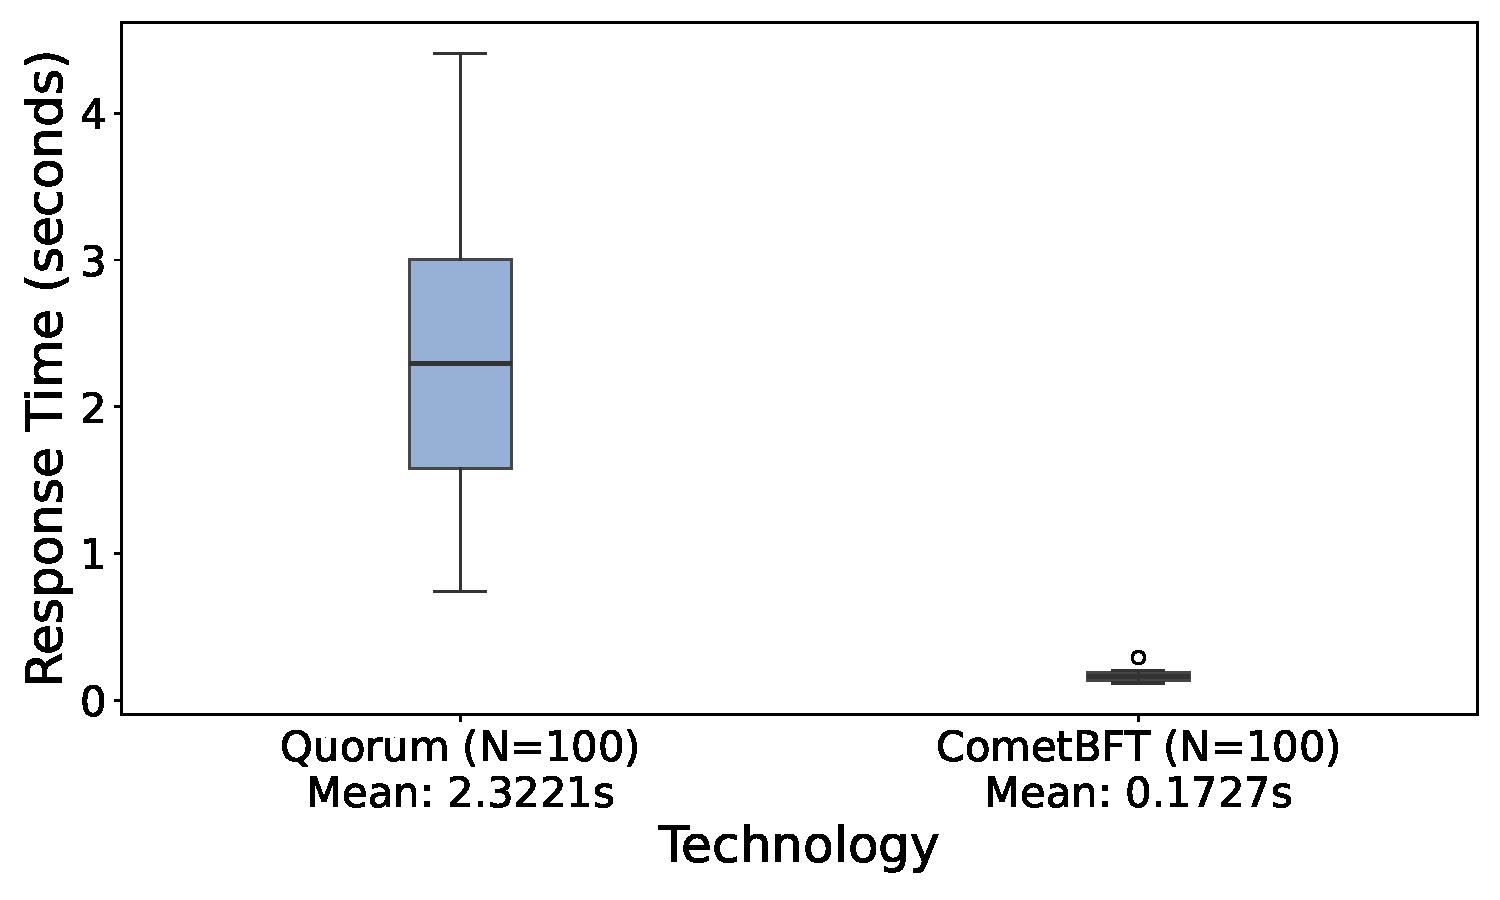
\includegraphics[width=0.72\textwidth]{Figures/Response_Time.pdf}
  \caption{Distribution of end-to-end response times in seconds under low traffic conditions for CometBFT and GoQuorum, over $100$ isolated-alert runs per backend. The mean response time is reported under each label.}
  \label{fig:resp_boxplot}
\end{figure}

Figure~\ref{fig:resp_boxplot} compares the distribution of end-to-end response times for the two configurations. The $x$-axis reports the evaluated technology together with its mean response time, while the $y$-axis reports the measured response time in seconds; for each configuration the box spans the interquartile range, the central line marks the median, and the whiskers represent the spread of the observations.

The results show a clear separation. CometBFT achieves a mean latency of $0.1727$\,s versus $2.3221$\,s for GoQuorum, an average response time roughly thirteen times lower. CometBFT also exhibits a markedly narrower interquartile range and a smaller overall spread, indicating more stable response times across runs, whereas GoQuorum shows both higher latency and greater variability. These results align with our prediction, GoQuorum's latency is bounded by all the tecnologic stack described in \chapter{requirement} such as the EVM and fixed minimum blocktime, CometBFT, by contrast, benefits from the on-demand block production, the first transaction is proposed immediately, the BFT round completes quickly on the validator set, and the state transition executes as a native Rust function call inside \texttt{DeliverTx} without bytecode interpretation or gas accounting.

From an SPS perspective this difference is both a performance and security relevant property. The liveness guarantee of Section~\ref{subsec:control_liveness} is bounded by the block production and execution latencies measured here, The experiment therefore empirically substantiates the qualitative claim that, under the sparse, event-driven alert traffic that characterizes a common SPS use case, CometBFT is lighter and more effective in supporting the requirements of the proposed architecture.


TODO DA QUI
% ==============================================================================
\section{Transaction Throughput under Increasing Load}
\label{sec:exp_throughput}
% ==============================================================================

% ------------------------------------------------------------------------------
\subsection{Motivation and Metric}
% ------------------------------------------------------------------------------

While Question~\ref{q:latency} characterizes the fixed cost per alert, Question~\ref{q:throughput} characterizes the variable cost under pressure. SPS workloads are not only sparse but also bursty: as noted in the burst-handling discussion of Chapter~\ref{chap:requirements} and in the deduplication rationale of Section~\ref{sec:impl_dedup}, a coordinated attack can trigger multiple IDS alerts within milliseconds, and a robust system must absorb these bursts without collapsing into unbounded latency or silently dropping alerts. The relevant metric is therefore the sustained transaction throughput of the ledger itself---the number of state transitions the consensus and execution layers can commit per unit of time---together with the latency required to drain a burst and the fraction of submitted transactions that are ultimately committed.

Throughput is a good metric for this comparison for two reasons. First, it stresses precisely the components that the requirement analysis flagged as divergent: the EVM execution and gas-metering loop that Quorum pays unconditionally, the fixed block period that bounds how quickly Quorum can drain its mempool, and, on the CometBFT side, the native ABCI execution path and the \texttt{CheckTx}-based mempool admission that allows the application to filter transactions before consensus (Section~\ref{subsec:impl_cometbft_app}). Second, it exposes the onset of performance degradation, which is where the architectural mismatch between a general-purpose platform and a narrow state machine becomes operationally visible: a backend that scales gracefully confirms that its overhead is intrinsic to the work being done, whereas a backend that collapses under load reveals overhead that is non-intrinsic and therefore, by the alignment lens of Section~\ref{sec:comparison}, a form of misfit.

\subsection{Experimental Design and Implementation}
\label{subsec:exp_throughput_design}

To evaluate the maximum throughput sustainable by the SPS, the harness progressively increases the input load by submitting transaction bursts ranging from $10^2$ to $10^5$ transactions, using up to $200$ parallel threads. For each burst size $N$ it measures (1) the number of transactions successfully committed to the blockchain, and (2) the elapsed time between the transmission of the first packet and the commitment of the last transaction. Throughput is then computed as the ratio between committed transactions and burst completion time, and the success rate as the ratio between committed and submitted transactions.

Two design choices are essential for fairness. First, the experiment injects transactions \emph{directly at the ledger's admission interface}, bypassing the IDS-to-member path, so that the measurement isolates raw ledger capacity rather than end-to-end attack handling; this is the regime in which the architectural difference between the two backends is cleanest. Second, the deduplication middleware of Section~\ref{sec:impl_dedup} is explicitly disabled on every node through the \texttt{POST /config/dedup} API for the duration of the benchmark, and the IDS alert path and the actuator feedback loop are muted. Disabling deduplication is necessary because its purpose is precisely to collapse redundant alerts into a single state transition; if it were active, the ledger would receive only a handful of transactions regardless of $N$, and the experiment would measure the middleware rather than the blockchain. Muting the IDS and the feedback loop prevents background traffic from contaminating the measurement. Both provisions are applied symmetrically and are reverted in a \texttt{finally} block at the end of the run, so that the lab is left in its default operating configuration.

The injection clients differ in transport but are matched in pressure. On CometBFT, a statically linked Rust binary (\texttt{sps-bench}) drives the validators through pipelined WebSocket \texttt{broadcast\_tx\_async} calls; on GoQuorum, a Node.js client (\texttt{quorum\_native\_bench.js}) drives the member nodes through concurrent \texttt{eth\_sendTransaction} calls with nonce resynchronization. Both use $200$ workers, a value well above each system's consensus throughput ceiling, so that the injection layer is never the bottleneck and the measured limit is genuinely the ledger's. After each burst the harness polls \texttt{/tx\_count} and the CometBFT \texttt{num\_unconfirmed\_txs} RPC until the chain reaches quiescence---a stable transaction count over several consecutive polls---before recording the final committed count and wall time; this ensures that transactions still in flight at the end of the burst are correctly accounted for rather than miscounted as lost.

\subsection{Results and Discussion}
\label{subsec:exp_throughput_results}

\begin{figure}[t!]
  \centering
  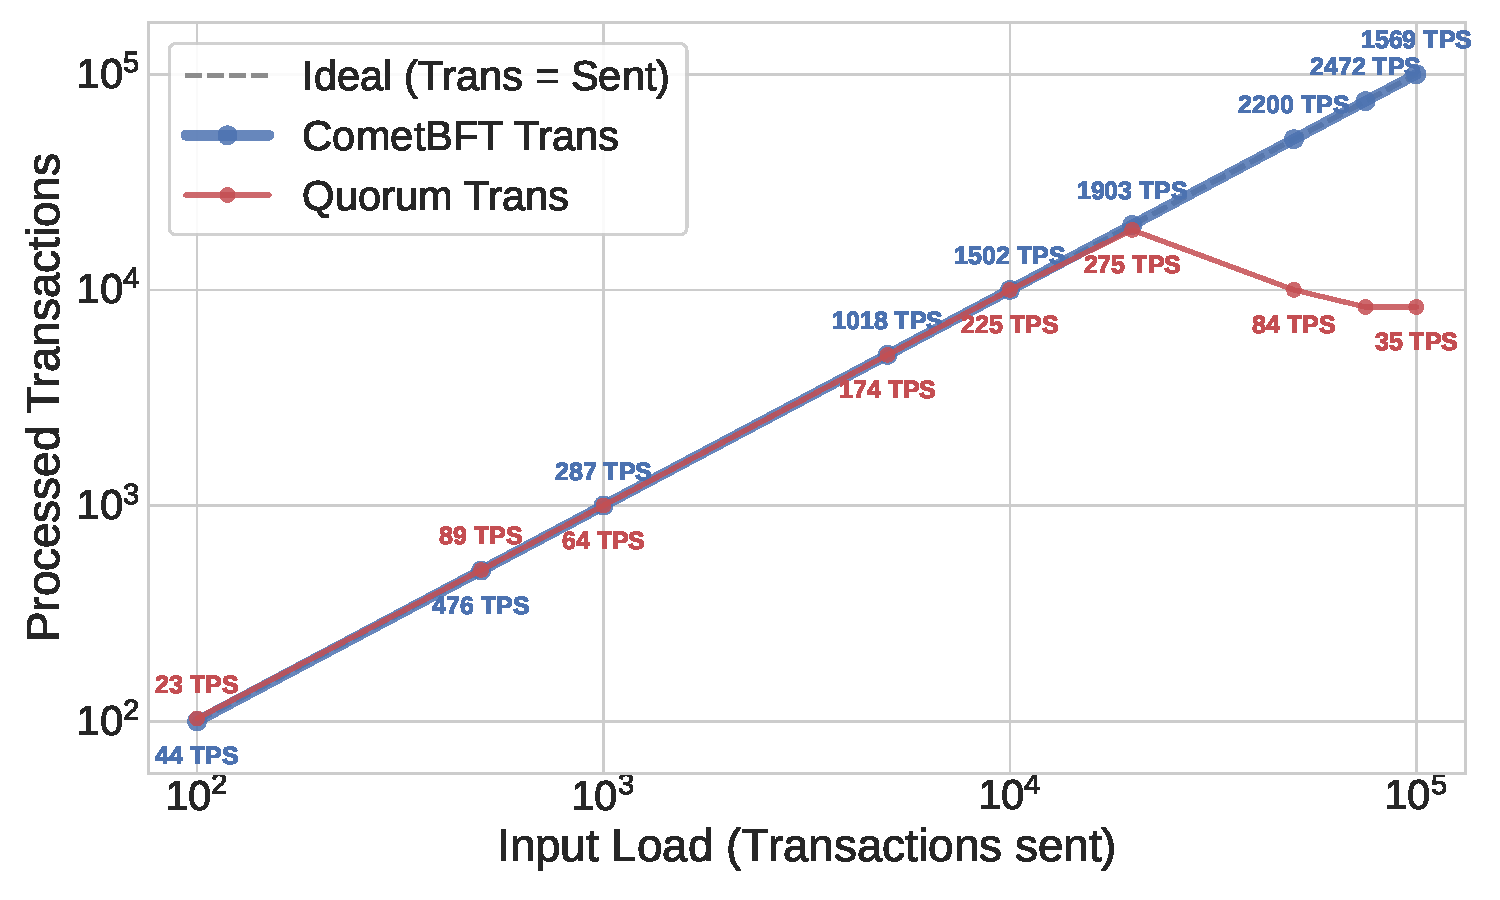
\includegraphics[width=0.78\textwidth]{Figures/comparison_transactions-1.pdf}
  \caption{Number of on-chain processed transactions as a function of the input load, on logarithmic axes, for the two blockchain configurations. The dashed diagonal is the ideal line (processed $=$ sent). Annotated values report the sustained throughput in transactions per second (TPS) at each load level.}
  \label{fig:throughput_trans}
\end{figure}

\begin{figure}[t!]
  \centering
  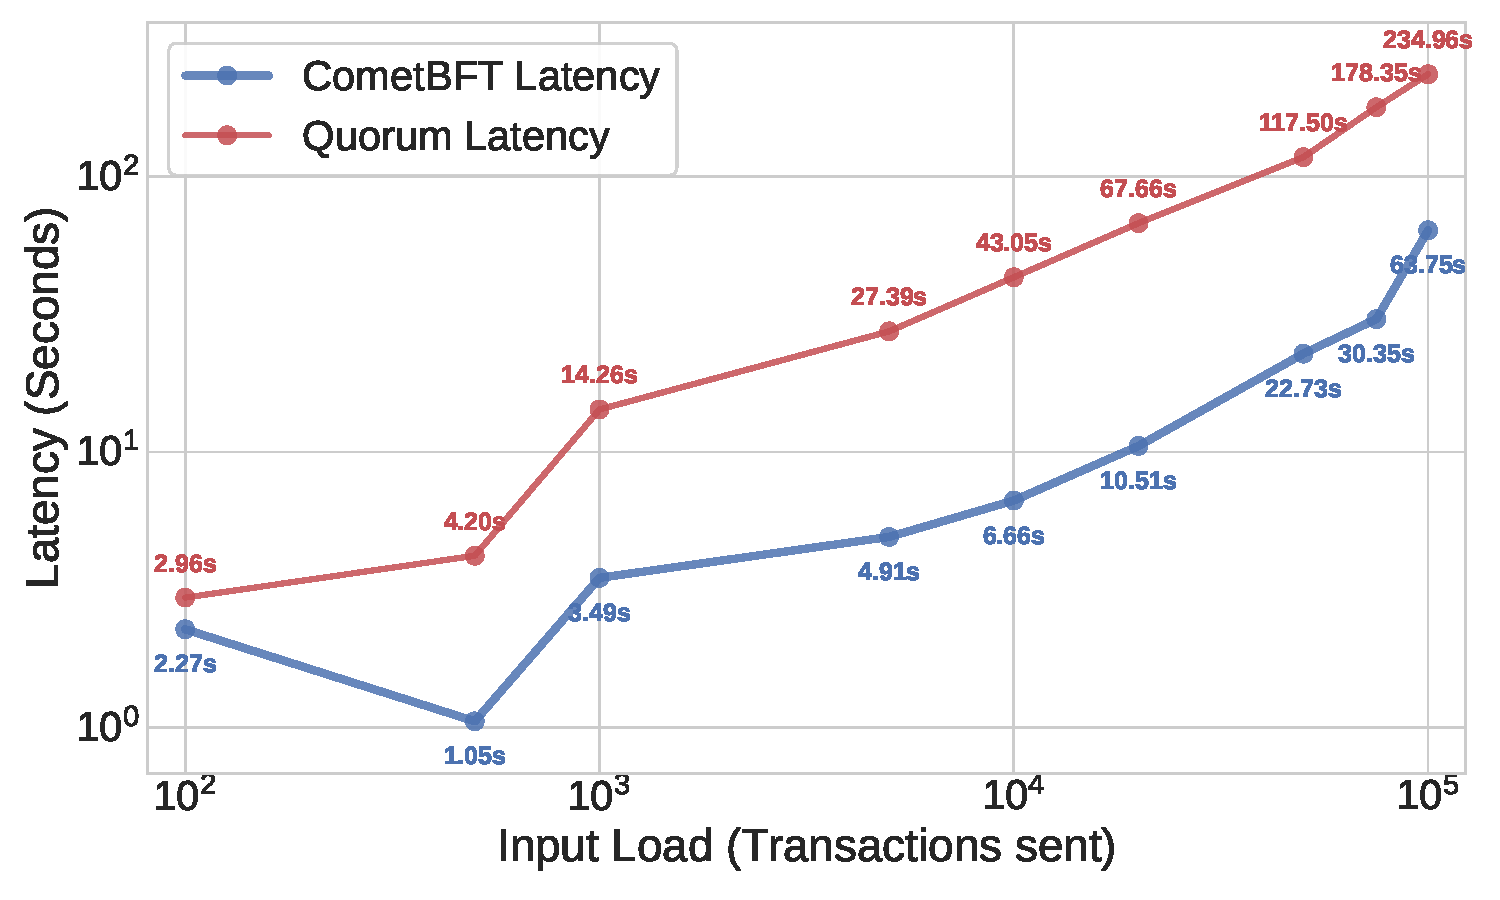
\includegraphics[width=0.78\textwidth]{Figures/comparison_latency.pdf}
  \caption{Burst completion latency as a function of the input load, on logarithmic axes, for the two blockchain configurations. Annotated values report the wall-clock time in seconds required to drain each burst.}
  \label{fig:throughput_lat}
\end{figure}

Figures~\ref{fig:throughput_trans} and~\ref{fig:throughput_lat} summarize the results from two complementary perspectives. Figure~\ref{fig:throughput_trans} reports, for each input burst, the number of transactions successfully committed on-chain against the ideal ``processed $=$ sent'' diagonal, annotating the sustained throughput in transactions per second (TPS); Figure~\ref{fig:throughput_lat} reports the wall-clock time required to complete each burst.

The results show a marked divergence. CometBFT scales effectively under increasing load: its committed-transaction curve tracks the ideal diagonal across the whole range, throughput rises from a few hundred TPS at low load to a peak of approximately $2.5$\,kTPS (the annotation reads $2472$~TPS) at the higher load levels, and no transaction loss is observed at any burst size. Latency grows accordingly from a few seconds to tens of seconds, reaching $63.75$\,s when submitting $100$\,K transactions, which is the expected price of draining a large burst through a fixed-size validator set with $O(n^2)$ voting communication (Section~\ref{subsec:validator_failure_quorum}). GoQuorum exhibits substantially weaker scalability. Throughput improves only under moderate load, peaking at approximately $275$~TPS for bursts of $20$\,K transactions, while latency increases sharply from seconds to several minutes, reaching $234.96$\,s at $100$\,K transactions---roughly $3.7\times$ the CometBFT figure for the same burst. At higher loads (above $10$\,K transactions) throughput collapses, with only about $10\%$ of submitted transactions successfully executed, and the committed-transaction curve detaches visibly from the ideal diagonal.

These outcomes map directly onto the requirement analysis. CometBFT's behaviour is consistent with the ``Execution model and deterministic state transitions'' discussion of Chapter~\ref{chap:requirements}: with the state machine implemented as a native Rust function inside \texttt{DeliverTx}, the per-transaction cost is proportional to the intrinsic logic of the transition rather than to virtual-machine scaffolding, and the \texttt{CheckTx} hook gives the application control over mempool admission. Combined with event-driven block production, this lets the ledger keep committing transactions as fast as the consensus round allows. GoQuorum's collapse is the empirical counterpart of the same analysis read in the opposite direction: every transaction pays RLP serialization, EVM bytecode interpretation, and instruction-granularity gas metering that execute unconditionally even though fees are zero; the fixed \texttt{blockperiodseconds=1} caps how quickly the mempool can drain; and once submissions outpace block production, the transaction pool fills and the success rate degrades. The higher CPU consumption observed on GoQuorum (Section~\ref{subsec:exp_resource}) is consistent with this interpretation: the extra cycles are consumed by the very machinery---gas accounting, EVM interpretation, on-chain governance---that the requirement table classifies as not needed.

From the SPS perspective, the decisive observation is not the raw peak throughput but the asymmetry in reliability under stress. CometBFT successfully executes \emph{all} submitted transactions across the entire range, whereas GoQuorum silently drops the majority of them once the load exceeds a few thousand transactions. In a self-protecting loop, a dropped alert is an unrecorded observation and, potentially, an unmitigated attack; a backend that sheds load by failing to commit transactions therefore undermines the liveness and auditability guarantees established in Sections~\ref{subsec:control_liveness}--\ref{subsec:act_safety}. The experiment thus corroborates, under sustained load, the same conclusion reached under low traffic: CometBFT better supports the SPS architecture, achieving higher throughput, lower delay, and---critically---no loss across all tested loads.

\subsection{Resource Consumption}
\label{subsec:exp_resource}

During the throughput benchmarks, user-process CPU utilization was monitored alongside the ledger metrics. On CometBFT, CPU utilization fluctuated between $9\%$ and $14\%$. GoQuorum exhibited slightly higher consumption, averaging $14\%$ and peaking at $17\%$. Although both figures remain modest in absolute terms---well below the $20\%$ ceiling observed throughout the campaign---the consistent gap is consistent with the architectural reading of Chapter~\ref{chap:requirements}: GoQuorum's higher resource usage is the runtime cost of the general-purpose virtual machine, gas accounting, and on-chain governance logic that the SPS does not need but cannot avoid, while CometBFT confines the trusted computing base to a small native state machine. This is the same mechanism that drives the latency and throughput gaps above, observed here in the dimension of energy and compute rather than time.

% ==============================================================================
\section{Effectiveness of the Deduplication Middleware}
\label{sec:exp_dedup}
% ==============================================================================

% ------------------------------------------------------------------------------
\subsection{Motivation and Metric}
% ------------------------------------------------------------------------------

The two previous experiments characterize the blockchain layer in isolation: Question~\ref{q:latency} at the single-alert extreme and Question~\ref{q:throughput} at the saturation extreme. The third experiment returns to the operating regime that the SPS actually faces in production---a regime in which a single sustained attack generates a large volume of redundant alerts that the system should not forward one-to-one to the ledger. As argued in Section~\ref{sec:impl_dedup}, a timed attack such as a sequence of SQL-injection attempts can produce hundreds of alerts per second, and three heterogeneous IDSs can each emit a matching alert within the same few milliseconds; since a BFT block commits on the order of seconds, the mempool would fill with thousands of redundant transactions describing the same state transition long before the first one commits, stalling consensus and inflating latency by orders of magnitude. The deduplication middleware was introduced precisely to prevent this, by dropping redundant alerts at the API level before they reach the mempool, since those redundant alerts would in any case be registered as a single response.

The metric of interest is therefore not throughput but \emph{compression}: how the number of transactions that actually reach the ledger scales with the volume of a specific attack, compared with the number of payloads sent, alerts detected, and alerts received at the blockchain-facing nodes. A good result is one in which the on-chain transaction count stays bounded---ideally constant---as the input load grows by orders of magnitude, while detection and ingress continue to scale. This directly tests the design goal stated in Section~\ref{sec:impl_dedup}: to keep the on-chain transaction load upper-bounded per block and per parameter, preventing mempool saturation while preserving the amount of information recorded. It also connects back to the broader architectural claim of Chapter~\ref{chap:requirements} that, in the SPS context, only state transitions matter and the relevant blockchain properties are minimality, determinism, and resilience rather than raw transaction capacity.

\subsection{Experimental Design and Implementation}
\label{subsec:exp_dedup_design}

Whereas Question~\ref{q:throughput} stresses the blockchain layer by disabling deduplication, this experiment enables it. The harness drives the attacker with \texttt{attacker\_burst.py} in \texttt{cycle} pattern, which sends the four canonical attack types (SQL injection, XSS, path traversal, command injection) in round-robin so that all four distinct state bits are exercised at every load level. The input load $N$ is progressively increased over four orders of magnitude. For each step the harness records four quantities:
\begin{itemize}
    \item \textbf{Sent}: the number of malicious payloads actually sent by the attacker;
    \item \textbf{Detected}: the number of alerts detected by the most virtuous IDS, taken as the maximum line count across the three IDS alert logs;
    \item \textbf{Ingress}: the sum of all alerts received at the blockchain-facing nodes, read from the \texttt{totalAlertsReceived} counter exposed by each node's \texttt{/stats} endpoint;
    \item \textbf{Transactions}: the number of transactions finally committed to the blockchain, read as the delta of \texttt{/tx\_count} between the beginning and the end of the run.
\end{itemize}

The experiment is run on the CometBFT configuration only. This is a deliberate, fairness-driven choice rather than an omission: with deduplication active, the number of transactions that reach consensus is so low that both backends behave equivalently, and a side-by-side comparison would measure experimental noise rather than an architectural difference. Focusing on a single backend keeps the figure legible while preserving the validity of the conclusion, which concerns the middleware rather than the consensus engine. Negative (recovery) alerts are suppressed for the duration of the run through a shared marker file consumed by \texttt{alert\_forwarder.py}, so that the deduplication cache is not reset between individual detections and the middleware can be observed over a sustained burst; between consecutive load steps, the harness sends a \texttt{SAFE\_ENVIRONMENT} reset to every light node, clearing both the ledger state vector and the per-node deduplication cache, so that each step starts from a clean baseline. Quiescence is enforced by polling \texttt{/stats} and \texttt{/tx\_count} until both stop growing before recording the final values.

\subsection{Results and Discussion}
\label{subsec:exp_dedup_results}

\begin{figure}[t!]
  \centering
  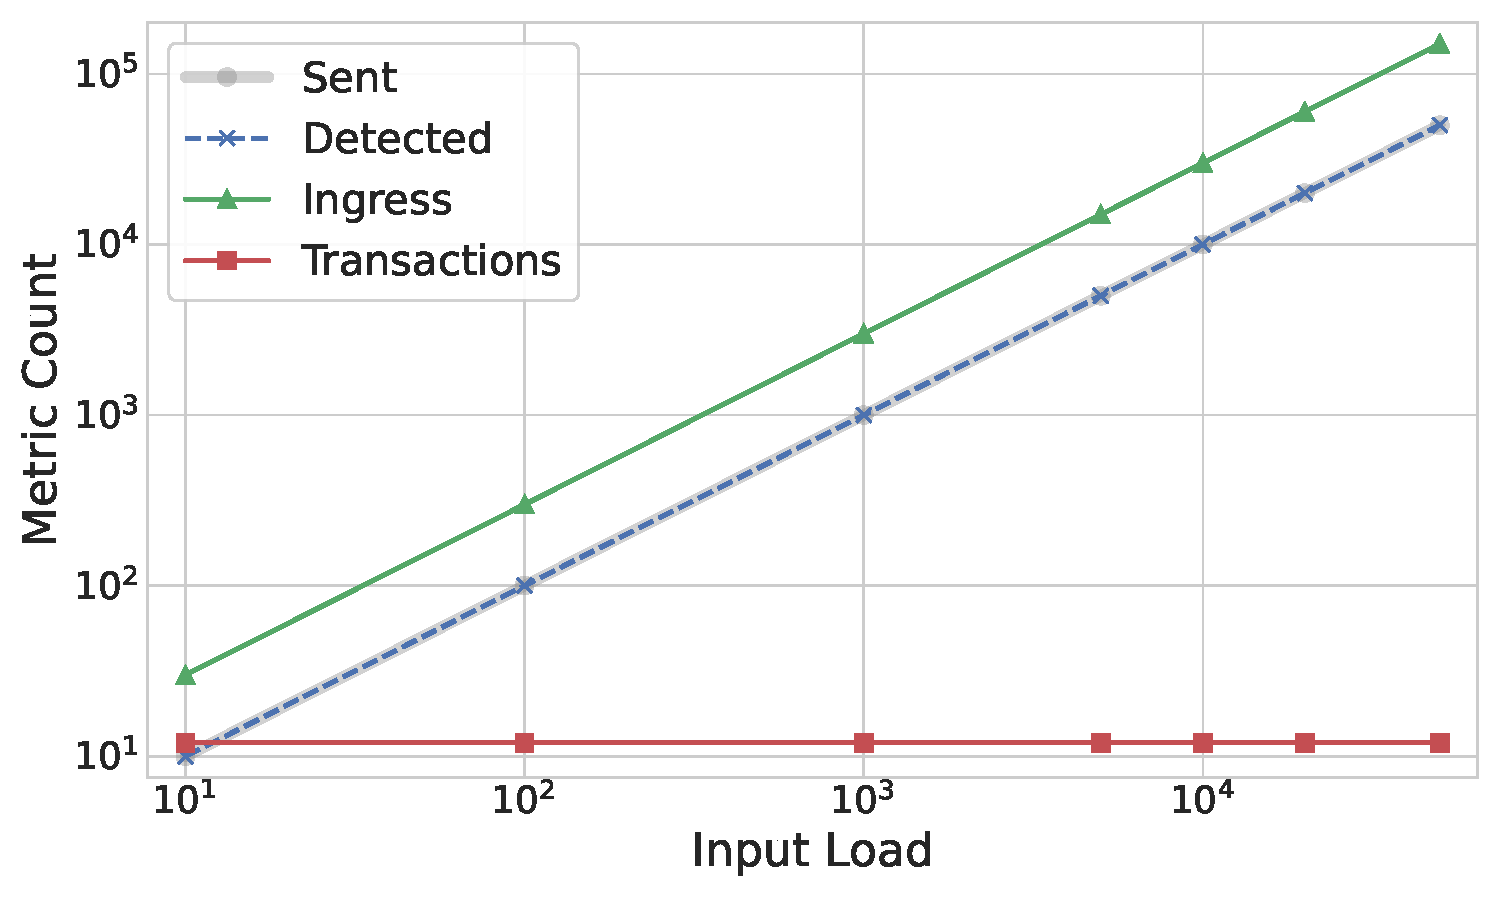
\includegraphics[width=0.75\textwidth]{Figures/SPS_comparison.pdf}
  \caption{Evolution of SPS processing metrics under increasing input load $N$, measured in attacks sent from the attacker machine: sent payloads, alerts detected by the most virtuous IDS, total ingress traffic received at the blockchain-facing nodes, and finalized blockchain transactions. Both axes are shown in logarithmic scale. Results are reported for the CometBFT configuration.}
  \label{fig:sps_dedup}
\end{figure}

Figure~\ref{fig:sps_dedup} is a multi-line plot showing how the four metrics evolve as the input load increases. The $x$-axis reports the input load $N$ and the $y$-axis the magnitude of each metric; both axes are logarithmic so that quantities differing by several orders of magnitude can be compared directly.

The results show that \textbf{Sent}, \textbf{Detected}, and \textbf{Ingress} all increase approximately proportionally with the input load, indicating that the attack-generation and detection stages scale consistently over the explored range and that the alert-forwarding path delivers the alerts to the blockchain-facing nodes without loss. In sharp contrast, \textbf{Transactions} remains essentially constant---flattening onto a single horizontal line on the logarithmic plot---even as the input load grows by four orders of magnitude. In the prototype this constant is bounded by the structural maximum $N_{\text{IDS}} \times N_{\text{types}} = 3 \times 4 = 12$ distinct state changes per step, which the middleware never exceeds regardless of how many redundant payloads the attacker produces.

This behaviour confirms the effectiveness of the deduplication middleware and closes the loop with several earlier claims. First, it validates the design rationale of Section~\ref{sec:impl_dedup}: because the consolidated state is a bit-vector and the response logic is a state--action map, any number of temporally adjacent alerts that request the same state change collapse into a single on-chain transition, so forwarding them individually would waste consensus cycles without altering the system's behaviour. By filtering redundant alerts at the API level before the mempool, the middleware keeps the on-chain load bounded per block and per parameter, which is exactly the property that prevents the mempool-saturation failure mode that Question~\ref{q:throughput} would otherwise expose. Second, it provides the operational complement to the requirement analysis of Chapter~\ref{chap:requirements}: the SPS does not need a high-throughput general-purpose ledger because the deduplication middleware, by exploiting the semantics of the state machine, ensures that the ledger is asked to commit only the transitions that actually matter. In this sense the experiment reframes the throughput result of Section~\ref{sec:exp_throughput}: CometBFT's multi-kTPS capacity is valuable not because the SPS routinely saturates it, but because it provides ample headroom above the bounded, deduplicated transaction rate that the system actually generates, so that even a misconfigured or partially defeated middleware is unlikely to stall consensus. Finally, the constant-transaction result confirms that the architecture preserves the full information content of the attack---which type occurred, confirmed by a quorum of heterogeneous IDSs---while shedding its redundant volume, which is the balance between auditability and efficiency that the ``configurable audit immutability'' discussion of Chapter~\ref{chap:requirements} anticipated.

Taken together with the latency and throughput results, the deduplication experiment completes the empirical picture. The SPS control loop reacts in fractions of a second on isolated alerts (Q1), sustains multi-kTPS bursts without loss when redundancy cannot be filtered upstream (Q2), and---in its intended operating regime---collapses four orders of magnitude of redundant attack traffic into a bounded, constant number of state transitions (Q3). Across all three regimes the CometBFT-based configuration exhibits the lower latency, higher throughput, and more predictable resource usage that the requirement-driven analysis of Chapter~\ref{chap:requirements} predicted, providing quantitative support for the thesis that an application-specific distributed state machine is a better fit for a cyber-resilient Self-Protecting System than a general-purpose smart-contract platform.

% ==============================================================================
% CHAPTER 6: CONCLUSIONS
% ==============================================================================

\chapter{Conclusions and Future Work}
\label{chap:conclusions}

% Wrap up the thesis.

\section{Summary of Research Findings}
\label{sec:conc_summary}
% Reiterate the winner of the comparison and why general-purpose blockchains are sub-optimal.

\section{Limitations of the Study}
\label{sec:conc_limitations}
% Discuss scalability issues of BFT with many nodes and static membership limits.

\section{Future Directions}
\label{sec:conc_future_work}
% Propose testing on physical clusters, complex attack scenarios, and sharding.

\printbibliography
\end{document}